\documentclass{beamer}
\usetheme{Madrid}
\usecolortheme{default}
\usepackage[utf8]{inputenc}
\usepackage{tikz}
\usepackage{circuitikz}
\usepackage{array}
\usepackage{amsmath}
\usepackage[export]{adjustbox}
\usetikzlibrary{calc}
\usetikzlibrary{positioning,shapes.gates.logic.US}
\usetikzlibrary {positioning}
\usetikzlibrary {arrows.meta,automata,positioning,shadows}

\colorlet{beamer@blendedblue}{blue!60!black}


\title{Assignment 11}
\subtitle{Solution to GATE EC2017, question 43}
\author{Perisetti Sai Ram Mohan Rao}
\institute{IIIT Raichur}
\date{\today}

\AtBeginSection[]
{
  \begin{frame}
    \frametitle{Table of Contents}
    \tableofcontents[currentsection]
  \end{frame}
}

\begin{document}

\begin{frame}
\maketitle
\end{frame}

\section{Question}
\begin{frame}{Question}
The state diagram of Finite State Machine (FSM) desgined to detect an overlapping sequence of three bits as shown in figure. The FSM has an input 'In' and an output 'Out'.The intial state of FSM is $S_0$ .

\begin{figure}[h]
\centering
\scalebox{0.5}{
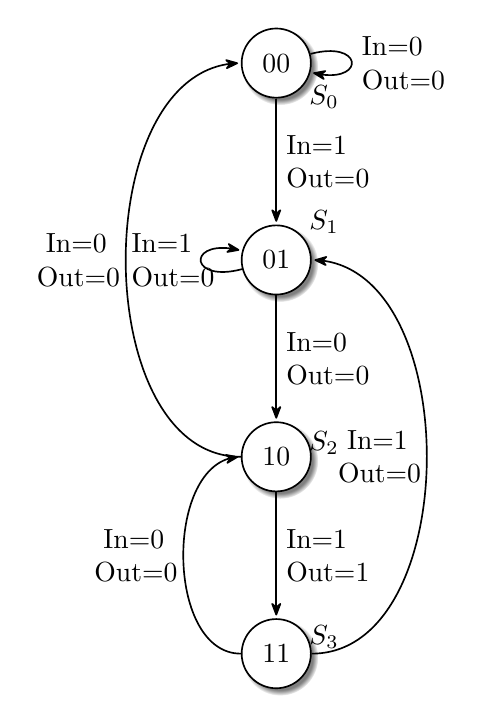
\begin{tikzpicture}[->,>={Stealth[round]},shorten >=1pt,auto,node distance=2.5cm,on grid,semithick,
every state/.style={fill=white,draw=black,circular drop shadow,text=}]
\node[state] (A)               {00};
\node[state] (B) [below =of A] {01};
\node[state] (C) [below =of B] {10};
\node[state] (D) [below =of C] {11};
\put (12,-15) {$S_0$};
\put (12,-60) {$S_1$};
\put (12,-140) {$S_2$};
\put (12,-210) {$S_3$};




\path (A) edge [loop right]   node[text width=0.75cm,align=center]{In=0\\Out=0}(A)
      (A) edge                node[text width=0.75cm,align=center]{In=1\\Out=0} (B)
      (B) edge [loop left]   node[text width=0.75cm,align=center]{In=1\\Out=0} (B)
      (B) edge                node[text width=0.75cm,align=center]{In=0\\Out=0} (C)
      (C) edge                node[text width=0.75cm,align=center]{In=1\\Out=1} (D)
      (D) edge [bend left=90]    node[text width=1.00cm,align=center]{In=0\\Out=0} (C)
      (C) edge [bend left=90] node[text width=1.0cm,align=center]{In=0\\Out=0} (A)
      (D) edge [bend right=90] node[text width=1.0cm,align=center]{In=1\\Out=0} (B);


\end{tikzpicture}}
\caption{}
\label{figure 1}
\end{figure}

If the input sequence is 10101101001101, starting with leftmost bit,then how many number of times 'Out' will be 1 is \rule{2cm}{0.10mm}
\end{frame}

\section{Solution}

\subsection{Pretext}
\begin{frame}{Solution / Pretext}
We are requried to find output sequence of Finite State Machine(FSM) and number 1's in output sequence.

\begin{figure}[h]
    \centering
    \scalebox{0.6}{
    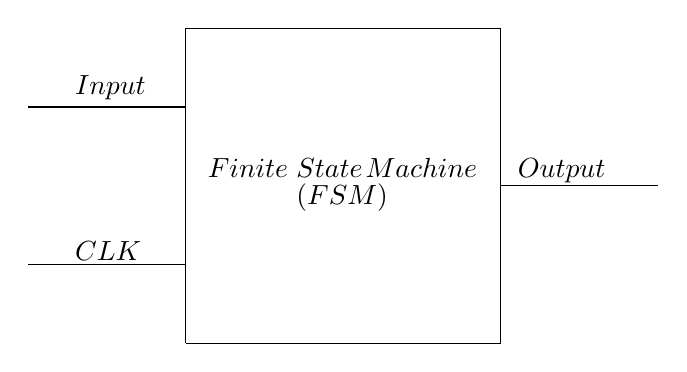
\begin{tikzpicture}

\draw (0,1)--(-2,1);
\draw (0,3)--(-2,3);
\draw (0,0) -- (4,0) -- (4,4) -- (0,4) -- (0,0);
\draw (4,2)--(6,2);
\put  (-40,90) {$Input$}
\put  (-40,30) {$CLK$}
\put  (8,60) {$Finite$}
\put  (40,60) {$State$}
\put  (65,60) {$Machine$}
\put  (40,50) {$(FSM)$}
\put  (120,60) {$Output$}

\end{tikzpicture} }
    %\caption{\textit{Question figure}}
    \label{fig:ques_}
\end{figure}
If the CLK is not applied,there will be no differnce between input sequence and the output sequence.

The mechanism that should take place in Finite state machine is mentioned in Figure 1.

\end{frame}

\subsection{Explanation}
\begin{frame}{Solution / Explanation}
\begin{columns}
\vspace{-0.05cm} % "\vspace" used to align picture vertically, preventing overflow
\column{0.5\textwidth}
\begin{figure}[h]
    \scalebox{0.6}{
    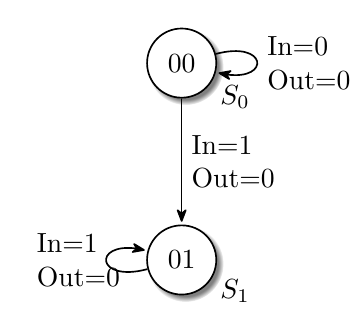
\begin{tikzpicture}[->,>={Stealth[round]},shorten >=1pt,auto,node distance=2.5cm,on grid,semithick,
every state/.style={fill=white,draw=black,circular drop shadow,text=}]
\node[state] (A)               {00};
\node[state] (B) [below =of A] {01};

\put (14,-15) {$S_0$};
\put (14,-85) {$S_1$};





\path (A) edge [loop right]   node[text width=0.75cm,align=center]{In=0\\Out=0}(A)
      (A) edge                node[text width=0.75cm,align=center]{In=1\\Out=0} (B)
      (B) edge [loop left]   node[text width=0.75cm,align=center]{In=1\\Out=0} (B);


\end{tikzpicture} }
    %\caption{\textit{Question figure}}
    \label{fig:ques_}
\end{figure}.
\column{0.5\textwidth}
In the finite machine we are requried to find the output in current state for corresponding input .We have to see Input value at current state to get the Output.For example if we are at current state $S_0$ with input=1 then Output =0 and state changes to $S_1$.
\end{columns}
\end{frame}

\subsection{Explanation}
\begin{frame}{Solution / Explanation}
\begin{columns}
\vspace{-0.05cm} % "\vspace" used to align picture vertically, preventing overflow
\column{0.5\textwidth}
\begin{figure}[h]
    \scalebox{0.6}{
    \begin{tikzpicture}[->,>={Stealth[round]},shorten >=1pt,auto,node distance=2.5cm,on grid,semithick,
every state/.style={fill=white,draw=black,circular drop shadow,text=}]
\node[state] (A)               {00};
\node[state] (C) [below =of B] {10};
\put (12,-20) {$S_0$};
\put (12,-160) {$S_2$};




\path (A) edge [loop right]   node[text width=0.75cm,align=center]{In=0\\Out=0}(A)
      (C) edge [bend left=90] node[text width=1.0cm,align=center]{In=0\\Out=0} (A);


\end{tikzpicture} }
    %\caption{\textit{Question figure}}
    \label{fig:ques_}
\end{figure}.
\column{0.5\textwidth}
We are now looking at another example.If the current state of FSM is $S_2$ with input=0
then it gives output=0 and state changes to $S_0$.

We are requried to find complete output sequence of FSM as stated in question.Which is made a table in next slide.  

\end{columns}
\end{frame}
\subsection{Conclusion}
\begin{frame}{Solution / Conclusion}
    \begin{table}[h]
    \centering
    \scalebox{0.8}{
    \begin{tabular}{|c|c|c|c|c|c|c|c|c|c|c|c|c|c|c|c|}
\hline
\textit{\textbf{Current State}} &\textit{\textbf{$S_0$}}  & \textit{\textbf{$S_1$}} & \textit{\textbf{$S_2$}} & \textit{\textbf{$S_3$}}&\textit{\textbf{$S_2$}} &\textit{\textbf{$S_3$}} &\textit{$S_1$} &\textit{$S_2$} &\textit{$S_3$} &\textit{$S_2$} &\textit{$S_0$} &\textit{$S_1$} &\textit{$S_1$}&\textit{$S_2$}  \\\hline
\textit{\textbf{Input}}         &    1                   &    0                    &   1                     &   0                    &   1                    &   1                    &   0            &   1           &   0           &   0           &   1           &   1           &   0          &    1            \\\hline
\textit{\textbf{Output}}        &    0                   &    0                    &   1                     &   0                    &   1                    &   0                    &   0            &   1           &   0           &   0           &   0           &   0           &   0          &    1           \\\hline
\end{tabular}}
    \caption{Table for States,Input and Output of finite state machine}
    \label{table}
\end{table}

The Output sequence of FSM is 00101001000001 from Table 1. \\
Then number of times 'Out' will be 1 is 4

\centering 
Answer = 4

\end{frame}

\section{Annexure}

\begin{frame}{Annexure}
    The behavior of state machines can be observed in many devices in modern society that perform a predetermined sequence of actions depending on a sequence of events with which they are presented. \\
    Vending machines, which dispense products when the proper combination of coins is deposited.\\
    Elevators, whose sequence of stops is determined by the floors requested by riders \\
    Traffic lights, which change sequence when cars are waiting. \\
    Combination locks, which require the input of a sequence of numbers in the proper order.
    
\end{frame}

\begin{frame}
    \centering
    \textit{Thank you.}
\end{frame}

\end{document}